\documentclass{article}
\pdfpagewidth=8.5in
\pdfpageheight=11in
% \usepackage{ijcai18}
% \usepackage{times}
\usepackage{xcolor}
\usepackage{soul}
\usepackage{amsmath,amsthm,amssymb,amsfonts,bbm}
\usepackage[noend]{algpseudocode}
\usepackage[utf8]{inputenc}
\usepackage[small]{caption}
% \usepackage{subfigure}
\usepackage[colorlinks]{hyperref}
\usepackage[a4paper,top=3cm,bottom=2cm,left=3cm,right=3cm,marginparwidth=1.75cm]{geometry}
% \usepackage[letterpaper]{geometry}
\usepackage[parfill]{parskip}
\usepackage[numbers, compress]{natbib}
\usepackage{hyperref}
\usepackage{subcaption}
\usepackage{wrapfig}
%\usepackage{xr-hyper,refcount}
\usepackage{natbib}
\usepackage{color,soul}
\usepackage{times}
\usepackage{latexsym}
\usepackage{amsmath}
\usepackage{changepage}
\usepackage{graphicx}

\usepackage{cleveref}
\usepackage{booktabs}
\usepackage{multirow}
\usepackage{makecell}
% \usepackage{algorithm,algorithmic}
\usepackage{mathtools}
\usepackage[normalem]{ulem}
\PassOptionsToPackage{numbers, compress}{natbib}

\definecolor{celadon}{rgb}{0.67, 0.88, 0.69}
\definecolor{salmonpink}{rgb}{1.0, 0.57, 0.64}
\definecolor{lightpink}{rgb}{1.0, 0.71, 0.76}
\definecolor{beaublue}{rgb}{0.74, 0.83, 0.9}
\definecolor{indianyellow}{rgb}{0.89, 0.66, 0.34}
\definecolor{lightapricot}{rgb}{0.99, 0.84, 0.69}
\newcommand{\hlc}[2][yellow]{{\sethlcolor{#1}\hl{#2}} }
\newcommand{\hlp}[2][beaublue]{{\sethlcolor{#1}\hl{#2}} }
\newcommand{\hln}[2][lightapricot]{{\sethlcolor{#1}\hl{#2}} }
% \definecolor{lightyellow}{rgb}{1.0, 1.0, 0.88}
\definecolor{lemonchiffon}{rgb}{1.0, 0.98, 0.8}
\newcommand{\hll}[1]{\hlc[lemonchiffon]{#1}}
\newcommand{\dd}[1]{\textcolor{red}{[  #1 -- Danish]}\typeout{#1}}

\title{
% \textbf{Beyond Accuracy: 
% } \\ 
Research Statement}
\author{Danish Pruthi\\
Language Technologies Institute\\
School of Computer Science\\
Carnegie Mellon University\\
\href{mailto:ddanish@cs.cmu.edu}{\nolinkurl{ddanish@cs.cmu.edu}}
}
\date{}

\begin{document}

\maketitle

\section{Introduction}

In the last decade, we have witnessed 
remarkable progress in natural language understanding,  
largely due to the resurgence of deep neural networks.
Supervised deep learning models 
boast impressive predictive abilities.
However, they remain \emph{uninterpretable} and are commonly treated as 
``black boxes''. 
% For many applications, 
% stakeholders desire not only predictions 
% but also \emph{explanations} or \emph{interpretations}
% for the purpose of assessing the 
% quality and morality of these predictions. 
% This ability to verify results engenders trust among users and 
% increases adoption of machine learning systems ~\cite{dzindolet2003role, herlocker2000explaining, ribeiro2016should}.
Researchers, practicioners, policy makers, and journalists have begun to express concerns that 
we must back our predictions by interpretations for the purpose of assessing the 
quality and morality of these predictions. 
Amidst growing concerns for interpretability, 
I am interested in the following questions:
\begin{itemize}
    \item How to supplement predictions with evidence that users can use to verify the validity of predictions? 
    \item How to evaluate the quality of a given explanation? 
    \item How to ensure (and measure the degree to which) an explanation is \emph{faithful} to the model? % being explained? 
\end{itemize}
Below, I outline some of the proposed and past research that aims to address these questions.
% Researchers, policy makers, and journalists have begun to express concerns that 
% we must supplement our predictions with interpretations for the purpose of assessing the 
% quality and morality of these predictions. 
% resulting in massive performance gains on several benchmarks. 

For many applications, 
end users desire not only predictions 
but also supporting evidence
so that they can readily verify the prediction.
% quality and morality of these predictions. 
This ability to verify results engenders trust among users and 
increases adoption of machine learning systems ~\cite{dzindolet2003role, herlocker2000explaining, ribeiro2016should}.
Fortunately, for many problems, a localized portion of the input
is sufficient to validate the predicted label. 
In a large image, a small patch of an image containing a hamster
may be sufficient to render the hamster label applicable. 
Similarly, in a long medical record, a single sentence may suffice
to identify a certain diagnosis.
For the task of evidence extraction,
we propose several new methods to combine 
scarce evidence annotations (strong semi-supervision) 
with abundant document-level labels (weak supervision).
% using both strong and weak supervision.
% The former takes the form of explicit, but scarce, 
% manual annotations of evidence segments,
% whereas the latter is provided by only input documents and their class labels.
% scarce evidence annotations (strong semi-supervision) 
% with abundant document-level labels (weak supervision) 
% (weak supervision)
% for the task of evidence extraction. 
% to jointly learn classifiers and evidence extractors.  
We find that our methods outperform 
% that feature evidence annotations,
% we find our methods to outperform 
baselines adapted from the interpretability literature 
to our task (refer to \S\ref{evidence} for details).
Our techinques
could potentially enhance 
explanatory information provided 
by
many Google services including Gmail, Ads, Search, etc. (Figure~\ref{fig:google},~\ref{fig:google_ads}).
% enable and enhance
    
\begin{figure}[h]
    \centering
    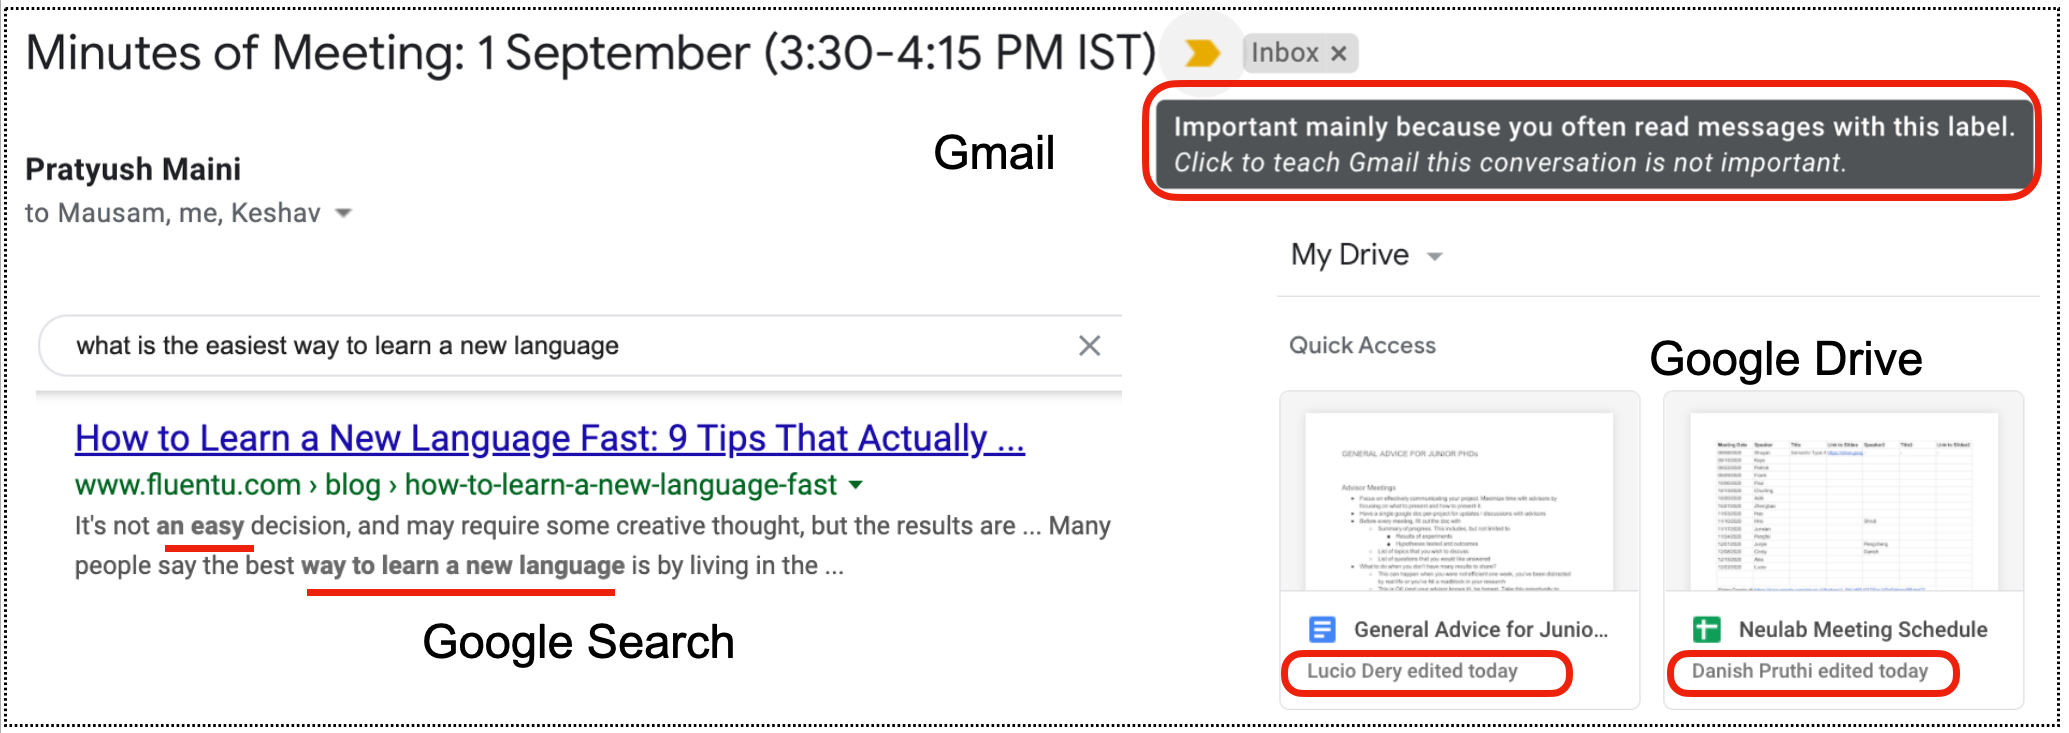
\includegraphics[width=0.99\textwidth]{google_v2}
    \caption{
    Several Google services provide some form of explanatory information. Top: Gmail Magic tool suggests why an email was marked important. 
    Bottom left: a search result highlights article tokens that are similar to the query tokens.
    Bottom right: the quick access tool offers brief reasons for the recommended documents in Google Drive.
    }
    \label{fig:google}
\end{figure}

Despite the large body of recent work on interpretability research (see xxx for a survey), 
there is little consensus on %on how to 
% many fundamental questions remain unanswsered. 
how to evaluate the quality of explanations.
To make matters worse, across papers,
the motives 
of intepretability 
% of interpretable models 
are diverse 
and occasionally discordant~\cite{lipton2018mythos}.
In an ongoing research effort (in collaboration with Google researchers) to alleviate these concerns, 
we propose a novel framework to assess the value of explanations.
Our framework draws upon the common use case of explanations---to \emph{communicate information
about how the decisions are made}, and thereby indicate how future decisions will be taken.
% explanations as a means of communication between a teacher and a student (which might be people or deep learning models).
We operationalize this usage 
via a teacher-student framework, where the teacher and the student could be humans or computer systems.
As per the framework, the goal of the student is to build a model that approximates the teacher's model
using the input, output, and explanations from the teacher.
Explanations provided by the teacher are effective if they help students predict better. 
Furthermore, the framework ensures 
that unfaithful explanations will not improve student's predictive ability (see \S\ref{communication} for more details).

\begin{figure}[t]
    \centering
    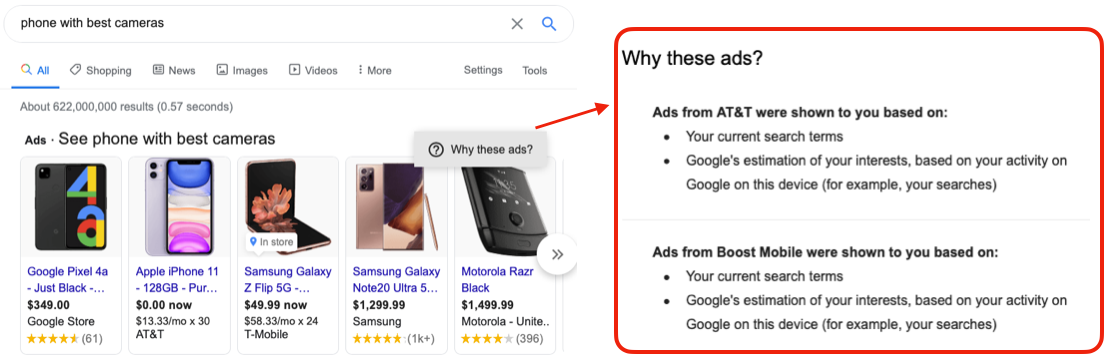
\includegraphics[width=0.95\textwidth]{google_ads}
    \caption{
     Why these ads? Partial explanations for the displayed advertisements.
    }
    \label{fig:google_ads}
\end{figure}

In a recent project, we also characterize the manipulability of popularly used attention-based explanations.


% \dd{Introduce other projects}.

\section{Ongoing and Past Research}

% In a series of papers over the past 2 years, I have pursued an expansive
% research agenda addressing multiple facets of
% interpretability in word representations~\cite{pruthi2018spine}, 
% robustness to subtle errors in text classification systems~\cite{pruthi2019combating}, 
% and reliability of attention-based explanation techniques~\cite{pruthi2019learning}. 

\subsection{Evidence Extraction} \label{evidence}
% \textit{How can we extract evidence using few evidence annotations (strong semi-supervision) 
% and abundant document-level labels (weak supervision)?}

Despite the success of deep learning for countless prediction tasks,
practitioners often desire 
that these models not only be accurate
but also provide \emph{interpretations} or \emph{explanations}~\cite{caruana2015intelligible, weld2019challenge}.
Unfortunately, these terms lack precise meaning,
and across papers, such explanations purport
% and papers on explanation purport 
to address such a wide spectrum of desiderata
that it seems unlikely any one method 
could address them all \citep{lipton2018mythos}.
In both computer vision \citep{ribeiro2016should, simonyan2013deep} 
and natural language processing \citep{lei2016rationalizing,lehman2019inferring}, 
proposed explanation methods often take the form of 
highlighting salient features of the input.
These so-called \emph{local explanations} are intended 
to highlight sets of features that elucidate 
``the reasons behind predictions'' %\cite{ribeiro2016should}.
However, this characterization of the problem remains under-specified.
Further, due to confounding, many features may be 
predictive but do not constitute \textit{evidence}~\cite{kaushik2019learning}.\footnote{For instance, in the IMDb movie review dataset 
the token ``horror'' is predictive of negative sentiment 
because horror movies tend to receive poorer ratings 
than movies from other genres~\cite{kaushik2019learning}.
However, no expert would mark it to be the evidence justifying the negative review.}
% Should we expand here?

Instead, we focus on supplementing 
predictions with 
%  not \emph{explaining} machine decisions, but rather unearthing
evidence that gives users the ability to quickly verify 
the correctness of machine predictions. 
% This ability to verify results engenders trust among users, 
% and increases adoption of the machine learning systems~\cite{dzindolet2003role, herlocker2000explaining, ribeiro2016should}.
Fortunately, for many problems, a localized portion of the input
is sufficient to validate the predicted label. 
Thus motivated, we cast our problem as learning to extract evidence
from both strong and weak supervision.
The former takes the form of explicit, but scarce, 
manual annotations of evidence segments,
whereas the latter is provided by only input documents and their class labels, 
which we assume are available in abundance.
% One way to view this problem is as a localization task
% that is fully-supervised vis-a-vis weak supervision
% and semi-supervised via strong supervision. 
In the extreme case where evidence annotations 
are available for all examples,
our task collapses to a standard multitask learning problem,
and in the opposite extreme,
where only weak supervision is available, 
we find ourselves back in the under-specified realm 
addressed by the interpretability literature.
% of rationale extraction. 

We optimize the joint likelihood of class
labels and evidence spans, given the input examples ($P(y, e | x)$)
We factorize our objective such that 
we first \emph{classify} ($P(y | x)$), and then \emph{extract} the evidence conditioned on the predicted label ($P(e | y, x)$).
For classification, we use 
BERT. %~\cite{devlin2018bert}.
The extraction task (a sequence tagging problem)
is modeled 
using a linear-chain CRF %~\cite{lafferty2001conditional} 
that takes representations and attention scores 
from BERT as emission features, 
allowing the two tasks to benefit from shared parameters.
Further, the evidence extraction module is 
conditioned on the predicted label, 
enabling the CRF to output different evidence spans 
tailored to the predicted class label.
This is illustrated in in Table~\ref{tbl:qual_example}. % for the task
% of sentiment analysis.% on movie reviews.

\begin{table}
    \small
    \centering
    \begin{tabular}{@{}c@{}}
    \toprule
     \textbf{Movie Review}                                                                                             \\ \toprule
     \begin{tabular}[l]{@{}l@{}} I don't know what movie the critics saw, but it wasn't this one. The popular consensus among newspaper \\ critics was that \hln{\textbf{this movie is unfunny and dreadfully boring}}. In my personal opinion, they couldn't be more wrong.\\ If you were expecting Airplane! - like laughs and Agatha Christie - intense mystery, then yes, this movie would \\ be a disappointment. However, if you're just looking for \hlp{\textbf{an enjoyable movie and a good time}}, this is \hlp{\textbf{one}} to see ... \end{tabular} \\ \midrule
    % $-$                      & \begin{tabular}[l]{@{}l@{}} I don't know what movie the critics saw, but it wasn't this one. The popular consensus among newspaper \\ critics was that  \hl{this movie is unfunny and dreadfully boring} . In my personal opinion, they couldn't be more wrong... \end{tabular}\\ \midrule \midrule
    \begin{tabular}[l]{@{}l@{}} Lean, mean, escapist thrillers are a tough product to come by. \hln{\textbf{Most are unnecessarily complicated}}, and others \\ have no sense of expediency--the thrill-ride effect gets lost in the \hln{\textbf{cumbersome}} plot. Perhaps the ultimate escapist\\ thriller was the fugitive, which featured none of the flash-bang effects of today's market but rather a bread-and-butter, \\ \hlp{\textbf{textbook example of what a clever script and good direction is all about.}} ... \end{tabular}\\ \midrule 
    % $-$                      & \begin{tabular}[l]{@{}l@{}} Lean, mean, escapist thrillers are a tough product to come by. \hl{Most are unnecessarily complicated}, and others \\ have no sense of expediency--the thrill-ride effect gets lost in the \hl{cumbersome} plot. Perhaps the ultimate escapist... \end{tabular}\\ \midrule 
    \end{tabular}
    \caption{Non cherry-picked evidence extractions from our approach. We condition our extraction model on both the \hlp{\textbf{positive}} and the \hln{\textbf{negative}} label. Our approach is able to tailor the extractions as per the conditioned label.}
    \label{tbl:qual_example}
    % \vspace{-0.2in}
\end{table}

% \gn{Is this the first work on evidence extraction? If so, then say so. If not, then you'll have to explain what's different.}

We directly compare our methods against
input attribution methods 
from the interpretability literature.
Many approaches in this category
first \emph{extract, and then classify}%~\cite{lei2016rationalizing,lehman2019inferring,jain2020learning,paranjape2020information}. 
% The classification task, by design,
% hinges on the extracted spans, 
% and hence a few of these approaches 
% 
% Some but not all of these methods 
% can be natually adapted to utilize abundant %document-level
% weak supervision~\cite{lehman2019inferring}.  
% 
% \gn{can't all of these methods use weak supervision? which ones can't? ``some'' is a bit deceptive.}.
Across two text sequence classification 
and evidence extraction tasks,
we find our methods to outperform 
baselines. Encouragingly, 
we observe gains by using our approach 
with as few as $100$ evidence annotations.



\subsection{Explanations as Communication}
\label{communication}

\begin{wrapfigure}{r}{4cm}
    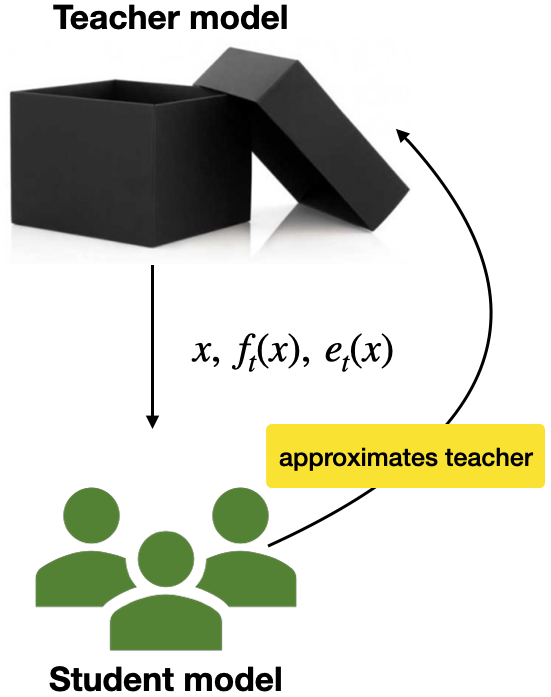
\includegraphics[width=4cm]{explanation-as-communication}
    \caption{Explanation as communication framework.}\label{fig:communication}
\end{wrapfigure} 
One familiar purpose of explanations for 
humans is to communicate information about 
how decisions are made, 
which also indicate how future decisions will be made.  
We formalize this specific 
use case of explanations:
%as the following task:  
assume a teacher $t$, a student $s$, and a series of inputs $x_1, \dots, x_n$, and 
suppose the student’s goal is to predict what the teacher will do in the future.
% this might be helpful in deciding who to trust in a leadership position, for instance.  
The student’s problem is thus a learning task, where the student needs to build a model $f_s(x)$ 
that approximates the teacher’s model $f_t(x)$.  
Explanations are modeled as 
additional side-information $e_t(x)$ that can be provided by the teacher in addition to label $f_t(x)$ for input $x$. 
Explanations are effective 
if a student can approximate $f_t(x)$ better or faster 
with explanations than with teacher-labeled examples alone. 
The degree by which different explanations 
help the student model 
provides a quantitative assessment 
of the value of explanations.
The above framework can be decomposed into two subproblems: 
i) for a teacher model $t$, how to obtain the explanatory information $e_t(x)$; and 
ii) how can the student model leverage this side-information $e_t(x)$ for training?

While the framework is broadly applicable, 
we apply it 
for question answering (QA) tasks.
We start with 
gold explanations 
collected 
from human experts.
Each explanation
contains 
necessary entities in the question and their relevant references in the passage.
We propose two new techniques 
to incorporate 
the explanation during training.
The first approach 
regularizes a (few) attention heads in a (few) layers 
to align with the symbolic mappings given by $e_t(x)$.
In the second method, 
we jointly 
predict i) the participating entities in the question and the passage using a linear-chain CRF~\cite{lafferty2001conditional},  
and ii) the start and end index of the answer span. 
For this multi-task
setup, we share the encoder representations
so that the task of QA would benefit from 
predicting 
the relevant entities.
We observe that regularizing
attention in such a manner results 
in an improvement of $6.4$ F1 points in the student QA model,
and jointly predicting entities and answers improves
the QA performance by $5.2$ F1 points.
Furthermore, 
we observe that student models perform better
with increasing quantity 
and quality of explanations.
These preliminary results
indicate that our framework
can be an effective  paradigm
to formalize the value of explanations. 
A 
more comprehensive
assessment of 
this framework 
is an active ongoing effort.




% This is still an ongoing effort, and these are only
% preiliminary results.

% Natural Questions (NQ) dataset.


\subsection{Manipulating Explanations}
\label{attention}

Since their introduction as a means to cope with
unaligned inputs and outputs in neural machine translation,
attention mechanisms 
have emerged as popular and effective components
in various
neural network architectures.
Attention works by aggregating a set of tokens via a weighted sum,
where the \emph{attention weights} are calculated 
as a function of both the input encodings and the state of the decoder. 
Because attention mechanisms allocate weight among the encoded tokens,
these coefficients are sometimes thought of intuitively
as indicating which tokens the model \emph{focuses on} 
when making a particular prediction. 
Based on this loose intuition, attention weights 
are often purported to \emph{explain} a model's predictions.
% Similar claims abound in the literature. 



In this study~\cite{pruthi19learning}, 
we elucidate two 
potential pitfalls  
why 
one should exercise caution in 
interpreting attention scores
as indicative of models' inner workings
or relative importance of input tokens.
First, 
we demonstrate  
that attention scores are surprisingly easy to manipulate 
by designing a training scheme 
whereby the resulting models appear to assign little attention 
to any among a specified set of \emph{impermissible} tokens
while nevertheless continuing to rely upon those features for prediction (see Table~\ref{tab:attn} for an example).
%a simple penalty term to the training objective. 
The ease with which attention can be manipulated
without significantly affecting predictions 
suggests that even if a vanilla model's attention weights 
conferred some insight (still an open and ill-defined question),
these insights would rely on knowing 
the precise objective 
on which models were trained.   
Second, 
practitioners often overlook the fact that
the attention is not over words 
but over final layer representations, 
which themselves capture 
information from neighboring words.
%We investigate this issue and other ways
% that models trained to produce deceptive masks 
% work around the constraints imposed by our training objective.
% To demonstrate these pitfalls, we design a training scheme 
% whereby the resulting models appear to assign little attention 
% to any among a specified set of \emph{impermissible} tokens
% while nevertheless continuing to rely upon those features for prediction. 
% We construct several of our tasks so that, by design, 
% access to the impermissible tokens are known to be essential
% in order to achieve high predictive accuracy.
% Unlike \newcite{jain2019analysis},
% who showed that attention maps could be (manually) manipulated 
% \textit{after} training without altering predictions,
% we interfere only with the training objective 
% and thus it is the \emph{actual} attention masks 
% produced by the resulting models
% that exhibit deceptive properties.
Our results present troublesome implications 
for proposed uses of attention in the context
of fairness, accountability, and transparency.
For example, malicious practitioners asked to justify 
\emph{how their models work} by pointing to attention weights
could 
mislead regulators with this scheme.

\subsection{Interpretable Representations}
\label{spine}

% We argue that this notion of interpretability can help in gaining better understanding of neural representations and models.
% Interpretability in a general neural network pipeline would not just help us reason about the outcomes that they predict, but would also provide us cues to make them more efficient and robust.
Distributed word representations (or word embeddings) are ubiquitous components of neural architectures applied in natural language processing. However, word embeddings are dense representations that people find difficult to interpret. For instance, we are often clueless as to what a high value along a given dimension of a vector signifies when compared to a low value. Here, our notion of interpretibility --- one that requires each dimension to capture a semantic concept --- is pragmatically motivated. In many classification problems, a linear (pre-softmax) layer projects representations hitherto to (un-normalized) class probabilities. Larger values of weights sway the output class probabilities greatly.  
% Weights from these linear layers bind to the final layer representation, and large positive and negative weights sway the output class probabilities. 
In order to explain a prediction, one necessarily has to understand the semantic concepts that each of the dimensions corresponding to these large weights represent. Hence, this notion of post-hoc interpretability is useful in explaining predictions.


% It is hard to interpret what raw values in individual dimensions signify -- we are often clueless as to what a `high' value along a given dimension of the vector signifies when compared to a `low' value.

To confer interpretability in word representations, we draw inspiration from various feature norming studies~\cite{garrard2001prototypicality,mcrae2005semantic}, where participants were asked to enumerate the properties of several words and concepts. It was observed that participants typically used few \emph{sparse} characteristic properties to describe the words, with limited overlap between different words. 
For instance, to describe the city of Pittsburgh, one might describe phenomena typical of the city, like erratic weather and large frequent bridges. It is redundant and inefficient to list negative properties, like the absence of the Statue of Liberty. Thus, sparsity and non-negativity are desirable characteristics of representations, that make them interpretable. 

We exploited these findings 
 to devise a novel denoising $k$-sparse autoencoder (see Figure~\ref{fig:autoencoder}) to obtain \textbf{SP}arse \textbf{I}nterpretable \textbf{N}eural \textbf{E}mbeddings (\textbf{\texttt{SPINE}}), a transformation of input word embeddings~\cite{pruthi2018spine}.
 % They are an extension of the $k$-sparse autoencoder (see Figure~\ref{fig:autoencoder}) that enforces sparsity and non-negativity constraints.
 These autoencoders are highly expressive, and facilitate learning of non linear transformations in contrast to linear matrix factorization. Further, they can be seamlessly integrated into a general neural network pipeline. Using our formulation, we attained representations that were twice as interpretable (as measured via intrusion detection tests) when compared to state of the art methods, with no loss in performance. 

 \dd{Add other projects}.


\begin{figure}[t]
\centering
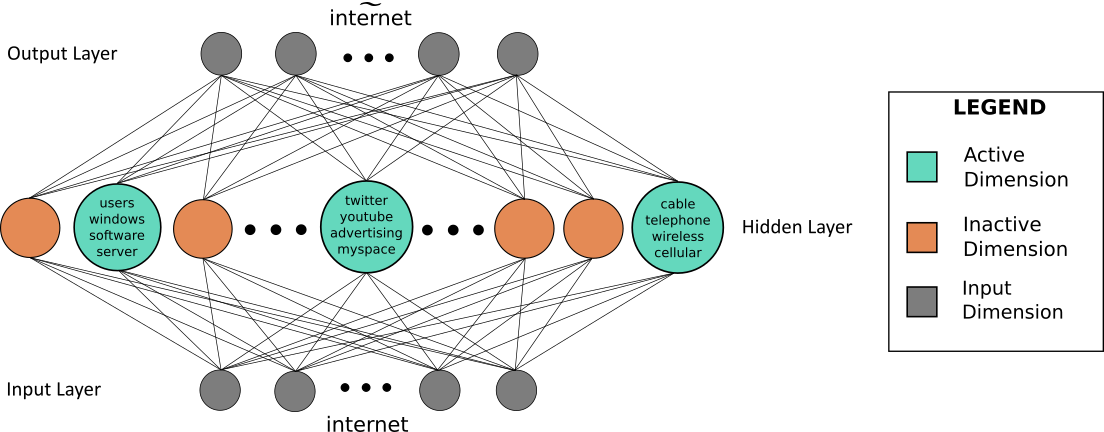
\includegraphics[width=0.70\textwidth]{autoencoder_detailed}
\caption{Depiction of our $k$-sparse autoencoder for an input word `internet'. Our variant of the $k$-sparse autoencoder attempts to reconstruct the input at its output layer,
with only a few active hidden units (depicted in green). These active units correspond to an interpretable set of dimensions associated with the word `internet'. The rest of the dimensions (depicted in orange) are inactive for this word.}
\label{fig:autoencoder}
\end{figure}


% \section{Proposed Work}
% \label{sec:proposed_work}




% Besides some of the initial work,

% It is widely believed that 
% eye-movements can help 

% I propose 
% to architect systems that capture, 
% and leverage auxiliary information 
% to cognitively understand and  
% mimick human reading and comprehension.
% Much of the stated auxiliary information is inherently
% produced but rarely
% recorded, like 
% eye movements, brain activity, etc.
% Some handy side-information can also be cheaply 
% gathered from human subjects upon follow up 
% prompts like requesting users to highlight relevant text portions, etc.
% Focusing on eye gaze information, I delineate my future plans to 
% i) examine cognitive processes of text comprehension (\S~\ref{subsec:scientific}) and  
% ii) supplement models with faithful 
% visual signals (from human eyes) 
% to align human and machine reading procedures, 
% resulting in greater accountability, and robustness (\S~\ref{subsec:engineering}). 



\bibliographystyle{plainnat}
\bibliography{refs}

\end{document}
